\documentclass[11pt]{article}

\usepackage{amsmath,amssymb,amsthm,setspace,tabto,fancyhdr,sectsty,mathtools}
\usepackage{titleps}
\usepackage[left=1.00in,right=1.00in,top=0.75in,bottom=1.50in]{geometry}
\usepackage{graphicx}
\graphicspath{ {assets/img/} }

% start pdfinlimg (GPLv3, https://github.com/zerotoc/pdfinlimg/blob/master/pdfinlimg.sty)
\newcommand{\pdfinlimg}[5]{
\makebox[#1cm][l]{\immediate\pdfliteral{
  q
  #3 0 0 #4 0 0 cm
  #1 0 0 #2 0 0 cm
  0.885 0 0 0.885 0 0 cm 
  BI
  /W #3
  /H #4
  /CS /RGB
  /BPC 8
  /F [ /AHx /Fl ]
  ID
  #5>
  EI
  Q
}\vbox to #2cm{}}
}
% end pdfinlimg

% BEGIN PARAGRAPH STUFF
\usepackage[utf8]{inputenc}
\usepackage[english]{babel}
 
\setlength{\parindent}{4em}
% \setlength{\parskip}{1em}
\renewcommand{\baselinestretch}{1}
% END PARAGRAPH STUFF

% useful commands
\DeclarePairedDelimiter{\ceil}{\lceil}{\rceil}
\DeclarePairedDelimiter{\floor}{\lfloor}{\rfloor}

\newpagestyle{footers} {
    \sethead{}{}{}
    \setfoot{\small Intro to Crypto and Blockchain, Note \notenum}{\thepage}{\small Rustie Lin}
    \footskip = 45pt
}

\fancypagestyle{firstpage} {
    \vspace*{3\baselineskip}
    \footskip = 0pt
    \renewcommand{\headrulewidth}{6pt}
    \chead{\rule{\textwidth}{6pt} \vspace{20pt}\\}
    \lhead{\setstretch{1.05}\Large\fontfamily{lmdh}\selectfont
    Introduction to Cryptocurrencies and Blockchain 
    \\ Lin, Akhtar}
    \rhead{\huge \fontfamily{lmdh}\selectfont    Note \notenum}
    \lfoot{\small Intro to Crypto and Blockchain, Note \notenum}
    \rfoot{\small Lin, Akhtar}
}
    
\sectionfont{\Large\fontfamily{lmdh}\selectfont}

% for initial paragraph indent
\usepackage{indentfirst}

% UPDATE THIS FOR EVERY NEW NOTE
\newcommand{\notenum}{2}

\pagestyle{footers}

\begin{document}
    \thispagestyle{firstpage}
    \vspace*{2\baselineskip}
    \section*{Bitcoin Protocol and Consensus: A High Level Overview}
    
    Often, underlying the excitement around Bitcoin, cryptocurrencies, and blockchain is a confusion about what exactly Bitcoin is and how it works at its core. This note is dedicated to explaining how Bitcoin works at a high level. 
    
    \section*{Bitcoin from the Ground Up}
    
    To fully understand how Bitcoin works, we start by attempting to build Bitcoin from scratch. Each time a major flaw is detected, a new feature must be built in. By the end of this section, we will have built Bitcoin from the ground up. Keep in mind that our goal is to create a currency that requires no central entity. Let us start off by considering two users of this currency, Alice and Bob.
    
    First step: establishing a system that allows users to write and sign messages describing transactions. Each transaction would be broadcast to the world (more specifically, every other user of the currency). If there exists no central third party to verify truths, then \underline{every other member of} \underline{the community becomes the third party}. For Alice to send Bob one bitcoin, she would announce to the world, ``I, Alice, am giving Bob one bitcoin," and the world would take note. A problem arises if Alice, intentionally or not, sends multiple identical messages to Bob. If she says five times in a row that she wants to give one bitcoin to Bob, did she accidentally repeat herself? Did she mean to send five bitcoins, or only one? The ability to send the same money multiple times would even give Alice the opportunity to spend more money than she has.
    
    To prevent ambiguity, we introduce uniquely identifiable serial numbers for each transaction conducted on the system. If Alice were to send one bitcoin to Bob now, she would announce ``I, Alice, am giving Bob one bitcoin with serial number \#\#\#\#." Modern banks use similar serial numbers to keep track of their transactions. If our version of Bitcoin were to implement serial numbers, it must need a centralized bank, a database or record to manage serial numbers, and thus transactions and balances. However, this defeats the purpose of a decentralized currency. 
    
    In trying to keep track of serial numbers, transactions, and balances, the centralized bank solution is undesirable, so naturally we aim to decentralize this feature. The solution is to make everyone the bank, giving everyone a complete record of all transactions. In this new scheme, Alice first sends Bob her transaction. Upon receiving the transaction, Bob then announces the transaction to the world, so that other users can update their records. What if Alice double spends on Bob and Charlie? In other words, if Alice sends the same bitcoin to Bob and Charlie, how does the system know which transaction is valid, if any? 
    
    Simply tracking transaction times is not valid, since in the realm of dropped packets and unreliable connections, network speed varies too much. To address this problem we edit the transaction sequence as follows: Alice sends a transaction to Bob, who then announces the transaction to the world. Everyone then verifies the transaction. This increases the security of the system, but it is still possible for Alice to double spend on Bob and Charlie. If she fabricates many fake online identities, she can then verify her own transaction with her other identities. In general,the attack pattern of creating many fake identities to subvert a system is called a \textbf{Sybil attack}
    
    To solve the Sybil attack issue of double spending, the system can implement a \textbf{proof-of-work} protocol to verify transactions. In a proof-of-work consensus system, when Alice wishes to make a transaction, she announces this to the entire network, as before. As others receive this message, they add to a \underline{list of pending transactions} that have yet to be verified. It should be noted that any user can maintain their own list of pending transactions, since they are not verified yet.
    
    To verify a list of pending transactions, an honest user --- call him David --- must do three things. First, he must check his version of the blockchain to ensure that the transactions in his list are valid (e.g. to check if the bitcoins involved have not been spent before.) Second, he must spend computation power to solve a difficult mathematical puzzle. Third, he must announce announce the list of transactions, now packaged into a new block, to the network. Other users in the system would then verify the transactions in the new block David has created, and append the new block onto the working blockchain.
    
    Arguably the most important step in this whole verification process, is the second, in which David must solve the math puzzle. By requiring David to solve this math puzzle, the system solves the problem of double spending. To analyze why this solves double spending, consider the case when Alice attempts to double spend with multiple identities. It is often difficult to identify dishonest actors in a network before they begin acting maliciously, as is the case with Alice. By requiring a mathematical puzzle to be solved, the system makes it costly for any user in the network to verify transactions. 
    
    A good way to understand proof-of-work is to view it as a competition. Users on the network are constantly in competition to verify their blocks of transactions. Malicious actors such as Alice are in constant competition with other users to verify transactions. As long as the majority of computational power is owned by honest users, then bad actors such as Alice will have difficulty double spending.
    
    In building the system from the ground up, we have highlighted the major features of Bitcoin. In the beginning, signed messages that are announced to the entire network formed the basis of the entire system. After adding serial numbers, the system was able to uniquely identify transactions. By making everyone in the network the "bank", we implemented a blockchain, allowing for a shared record of transactions. The idea of having everyone in the network verify transactions provided a much-needed increase in security. Finally, proof-of-work prevents malicious actors in the network from double-spending, allowing the system to be trustworthy. 
    
    \section*{Basic Concepts -- Identity in Bitcoin}
    
    As described earlier, one of the most fundamental concepts in Bitcoin is the idea of sending money between pseudonymns. In the form of cryptogrpahy employed by the Bitcoin system, a pseudonymn refers to a user's Bitcoin address or the hash of their public key. 
    
    Bitcoin also buids on some cryptographic primitives. Firstly, Bitcoin uses \textbf{ECDSA (Elliptic Curve Digital Signature Algorithm)} as its digital signature scheme. This allows for cryptographically secure public and private key pair functionality that bears similarity to username and password schemes. Additionally, Bitcoin uses a one-way cryptographic hash function called \textbf{SHA-256} in its proof-of-work scheme. As a cryptographic hash function, SHA-256 takes in an arbitrary amount of data, and deterministically creates an output of fixed size. Also, SHA-256 is one-way, meaning that for a given output, it is very difficult to find its corresponding input. A small change in the input data can completely change the output. These properties allow effective usage of SHA-256 in various parts of the Bitcoin network, including the proof-of-work scheme and also in the creation of bitcoin addresses.   
    
    Another key concept in Bitcoin is the idea that bitcoin is hidden in the large amount of public keys. Users in the Bitcoin network can generate arbitrarily many key pairs. The idea of owning bitcoin, as we will discuss later on, boils down to proving ownership of public keys or addresses. There $2^{260}$ possible addresses. To put this massive number into perspective, consider the following. There are roughly $2^{63}$ grains of sand on the Earth. Doubling the exponent, $2^{126}$ is actually only 0.0000000058\% of $2^{160}$. We only reach $2^{160}$ if we imagine that for each of the $2^{63}$ grains of sand on Earth, there is another Earth, each with its own set of grains of sand. The number of bitcoin addresses is so large that mathematically we can assume that the possibility of colliding with someone else's bitcoin whenever a user generates a public/private key pair is negligible. (For those curious, $2^{160}$ is exactly 1,461,501,637,330,902,918,203,684,832,716,283,019,655,932,542,976 -- \textit{Rustie}) 
    
    \section*{Transactions -- A Basic Version}
    
    Transactions are usually conducted through wallet software, although it is possible to do this manually. Wallet software automatically generates Bitcoin addresses for its users. Users can then receive money by sharing their addresses, or send money specifying an address and amount. In many online wallets, transactions can even be conducted easily via a series of QR codes (e.g. in the Coinbase interface.) Whenever a transaction is made, it is broadcast to the entire Bitcoin network, where miners verify the transaction and add it to the transaction history.
    
    \section*{Introduction to Transactions}
    
    When a user spends bitcoin, they are spending from previous transactions. Transactions are mappings from inputs to outputs, where inputs and outputs both each contain an address and an amount. In a typical transaction, in order for Bob to spend 0.05 BTC at a coffee shop, Bob could create a transaction with one input and two outputs. If the transaction input was 1.00 BTC, then the outputs would be 0.05 BTC to the coffee shop, and 0.95 BTC back to Bob. The reason for two outputs is because as per the Bitcoin system specification, inputs can only be spent once. Thus creates the need for a change output (the 0.95 BTC) back to the sender. Users of Bitcoin can also impose transaction fees by constructing transactions in such a way as to make the input amount and output amount sum up to different values. In the previous example, if Bob sends 0.05 BTC to the coffee shop and only 0.94 BTC back to himself, then the Bitcoin system will calculate the difference in inputs and outputs (1.00 BTC - 0.05 BTC - 0.94 BTC = 0.01 BTC). This is what bitcoin miners collect as transaction fees. 

   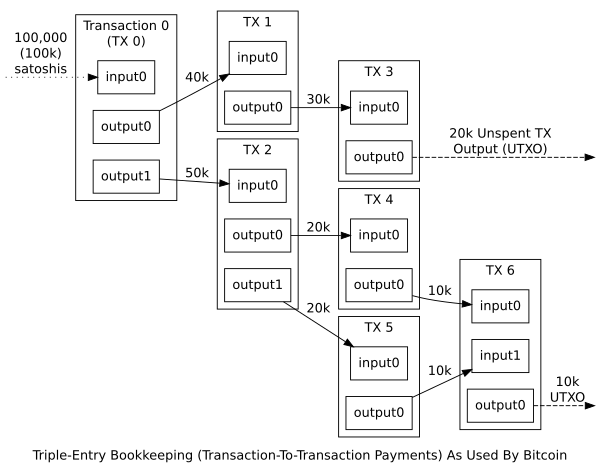
\includegraphics[scale=0.9]{note2_transactions}
    
    
    % BEGIN KEY TERMS
    \newpage
    \thispagestyle{firstpage}
    \vspace*{2\baselineskip}
    \section*{Key Terms}
    \noindent A collection of terms mentioned in the note which may or may not have been described. Look to external sources for deeper understanding of any non-crypto/blockchain terms.
    \begin{enumerate}
        \item \textbf{Sybil attack} --- A strategy by which a single entity generates additional identities, often a great many, in order to gain substantial undue influence in a peer-to-peer network. The rest of the network is not aware that all these identities belong to one person in a successful attack.
        \item \textbf{Proof-of-work} --- A piece of data which is costly to produce but easy for others to verify and which satisfies certain requirements. 
        \item \textbf{ECDSA} --- Short for \underline{E}lliptic \underline{C}urve \underline{D}igital \underline{S}ignature \underline{A}lgorithm. In Bitcoin, ECDSA is used to generate public and private key pairs, which in turn allows users to sign transactions such that third parties can verify the authenticity of the signature while retaining exclusive ability to create the signature.
        \item \textbf{SHA-256} --- A cryptographic hash function used in various parts of the Bitcoin network such as the proof-of-work challenge.
        
     
    \end{enumerate}
    % END KEY TERMS
\end{document}